
\chapter{Combine: Design Galleries}
\label{ch:hapticexamples}

\begin{figure}[htbp]
\begin{center}
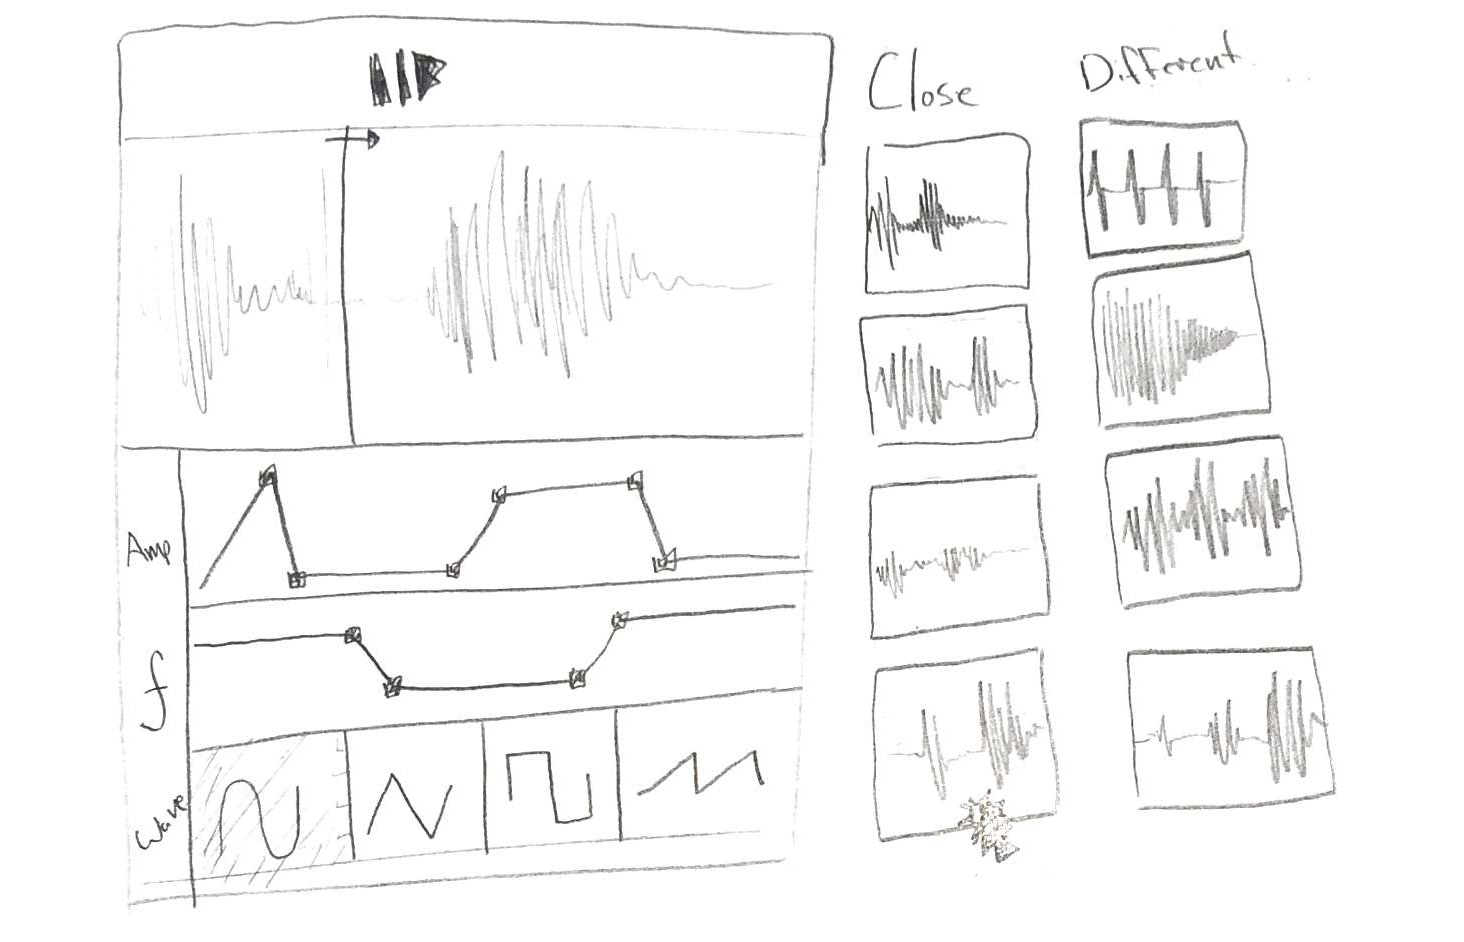
\includegraphics[width=4in, height=2.17in]{VTDesignGallerySketch}

\caption{Concept sketch for a vibrotactile design gallery.}
\label{hapticexamples:designgallerysketch}
\end{center}
\end{figure}

In both the Haptic Instrument and Tactile Animation case studies, participants drew from their experience or external examples and requested features for repetition.
This is unsurprising; creative tasks, like design, are often defined as the recombination of existing ideas, with a twist of novelty or spark of innovation by the individual creator \cite{Warr2005}.
Examples are critical to provide inspiration, guidance, and inform design \cite{Herring2009,Buxton2007}; for example,
%In other fields of design, designers clip, store, and display examples for inspiration \cite{Buxton2007}.
industrial designers collect various knobs and materials, and web designers bookmark sites \cite{Herring2009}.
Managing these examples effectively is already a significant task even in these more visual fields, but there is no explicit support for vibrotactile (VT) design.
I will investigate interaction techniques to directly use examples in haptic design through a design gallery tool for VT icons (\autoref{hapticexamples:designgallerysketch}).



Design galleries are used in graphics and web design to facilitate the use of examples \cite{Lee2010a,Marks1997}.
While there are several challenges involved with examples in design, including capture, search, management, use, and sharing, I limit this project's scope to the \emph{combining} existing examples to create new VT icons.
This project takes place in two phases: Phase I, where we develop a set of tools to manipulate VT icons through interpolation and combination, and Phase II, creating a design gallery and investigating how users work with it (or would like to, if they are unable to do so).
For this study, we use a single Haptuator bound to a mobile device to simulate mobile VT icons (\autoref{fig:macarondevice}).


%\begin{figure}[htbp]
%\begin{center}
%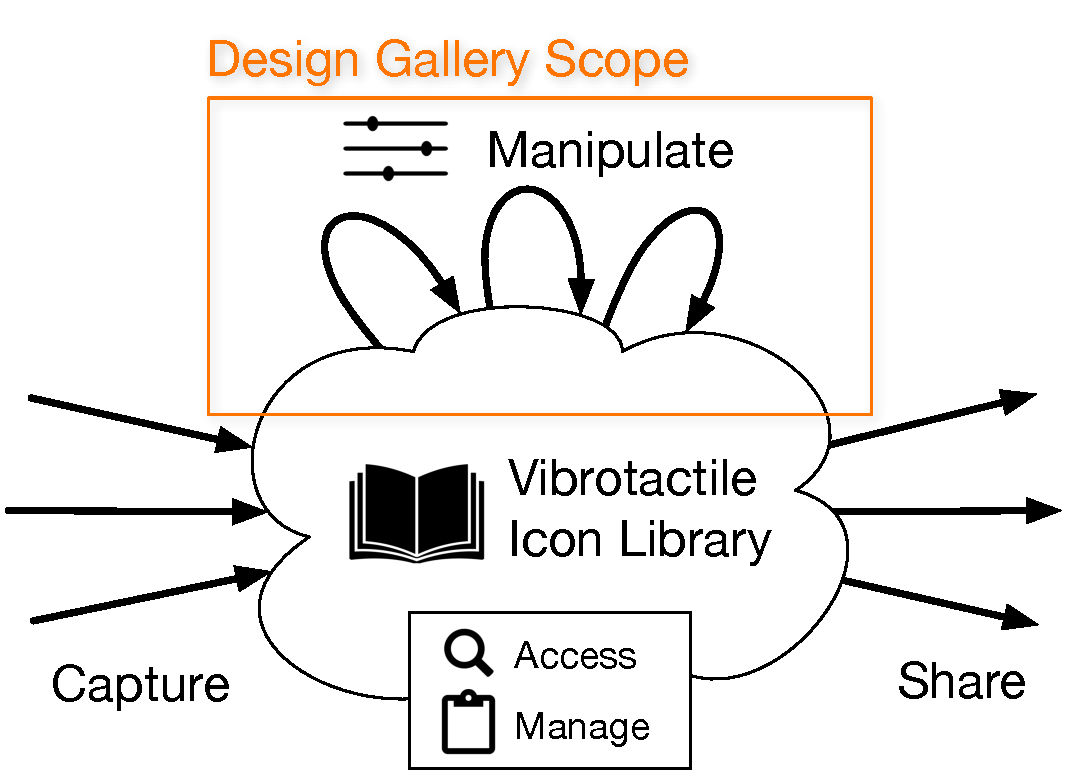
\includegraphics[width=0.4\textwidth]{ExamplesEcosystem}
%
%\caption{Example ecosystem and design gallery scope.}
%\label{hapticexamples:overview}
%\end{center}
%\end{figure}



\begin{figure}[htbp]
 \centering
   \begin{subfigure}[t]{0.35\textwidth}
	  \centering
	   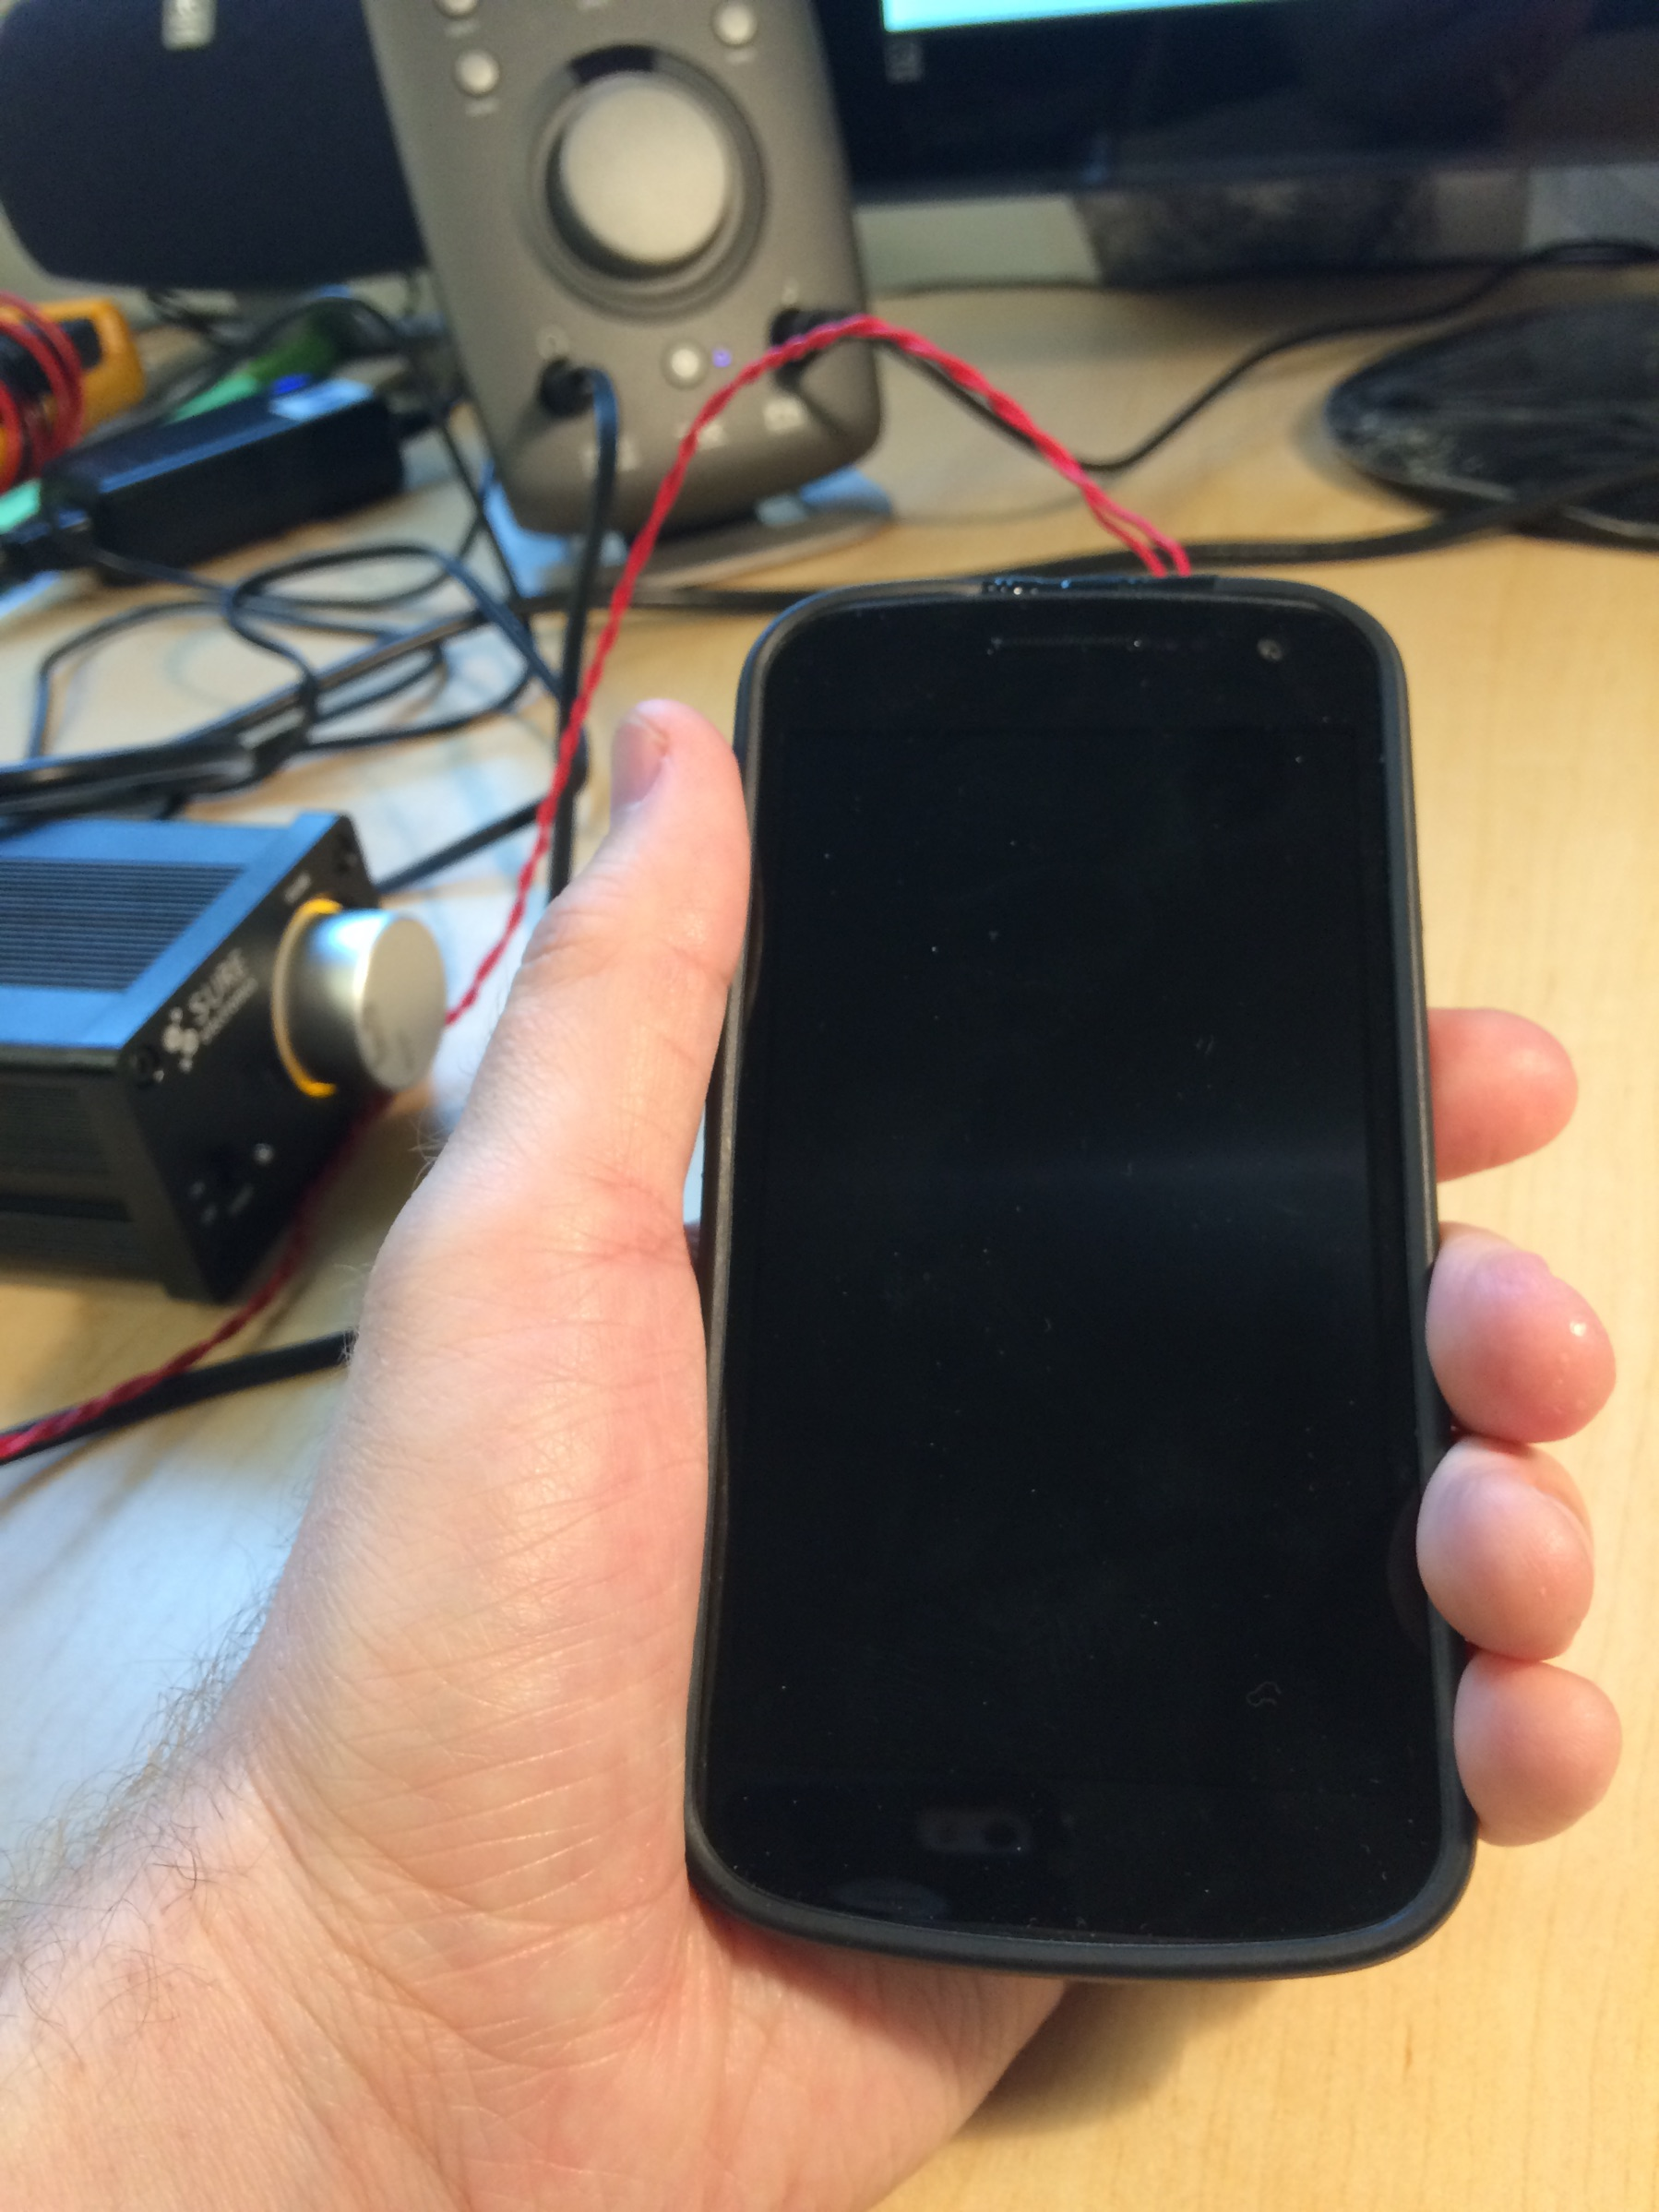
\includegraphics[width=\textwidth, clip=true, trim=0 200 0 0]{macaron-device1} 
	   \label{fig:macarondevice:front}
    \end{subfigure}
    \qquad
     \begin{subfigure}[t]{0.35\textwidth}
	  \centering
	   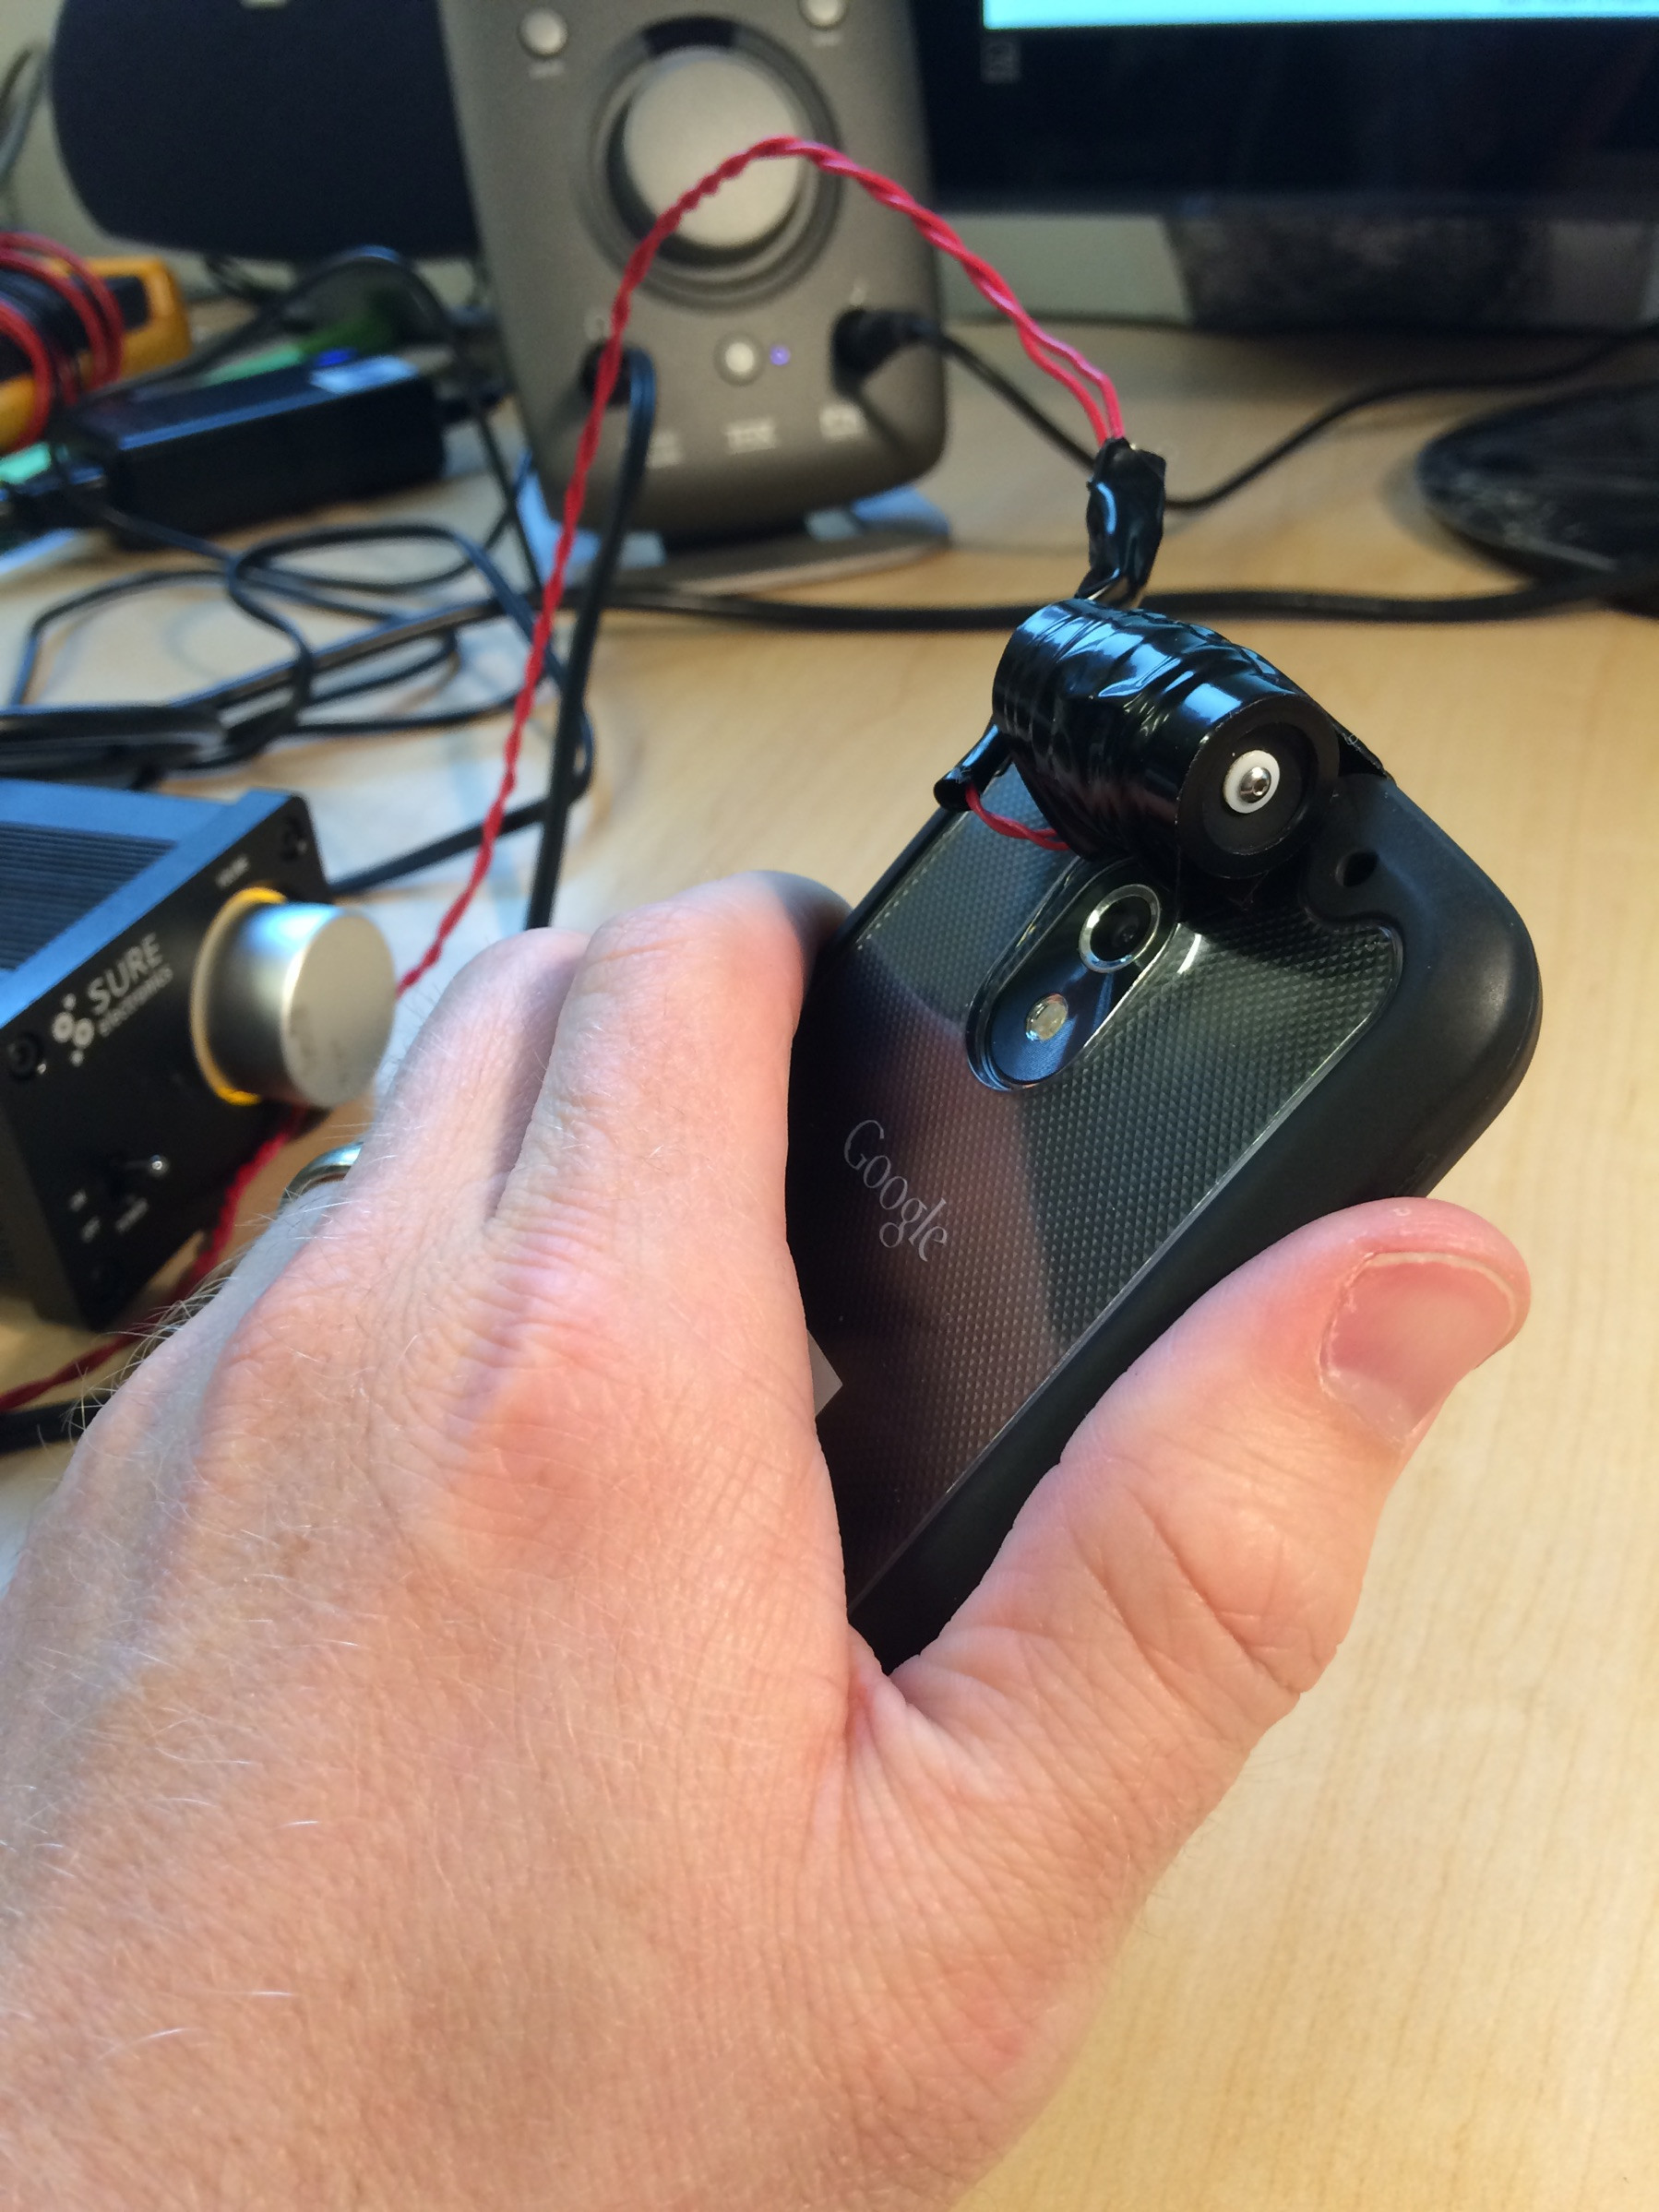
\includegraphics[width=\textwidth, clip=true, trim=0 200 0 0]{macaron-device2} 
	   \label{fig:macarondevice:back}
    \end{subfigure}

    \caption{Apparatus. A Haptuator is mounted onto a Galaxy Nexus smartphone to simulate mobile VT icon development, similar to \cite{InwookHwang2013}.}
    \label{fig:macarondevice}
\end{figure}


\section{Phase I -- Algorithms and Interaction Techniques}
In Phase I, I will develop and evaluate algorithms for manipulating examples by adjusting low-level parameters (frequency, amplitude, duration, and waveform), interpolating between examples, and combining aspects of different examples (for example, combining the frequency profile of one example with the amplitude profile of another). These algorithms will be evaluated using a perceptual study to examine two criteria: a smooth, linear interpolation method between VT icons, and to produce a varied corpus of VT icons.

\subsection{VT Icon Editing}
The design parameters of VT icons are already well understood to be frequency, amplitude, waveform, rhythm, and location.
In this study, we focus on a single actuator display.
Direct editing is supported with a track-based editor, similar to previous work \cite{Swindells2006}, using keyframes like those in the tactile animation prototype, Mango, with one track each for frequency, amplitude, and waveform.
These tracks constitute envelopes of each parameter over the duration of the VT icon.
Rhythm emerges as the amplitude envelope.
In order to use waveform as a time-varying parameter, we crossfade between phase-synchronized waveforms, as used with haptic knobs in \cite{MacLean2009a}.
As this would be the first instance of continuous, time-varying waveform as a VT design parameter, we validate using piloting.
A more thorough study would be valuable to the VT literature, but is secondary to our research questions about the design process.

\subsection{VT Icon Replacement}
In addition to directly editing parameters, we want to enable using examples directly in the design process.
By using a track-based approach to VT icons,  we get another interaction technique: full or partial replacement.
In a design gallery, users can select an icon as a starting point, which we call \emph{full replacement}.
However, tracks can also be replaced, as long as some normalization technique is applied to accommodate different durations.
This \emph{partial replacement} is a weak form of example-based design, where users can combine examples in a limited way to create a new VT icon.
A richer tool would be to more fluidly morph between icons.


\begin{figure}[htbp]
\begin{center}
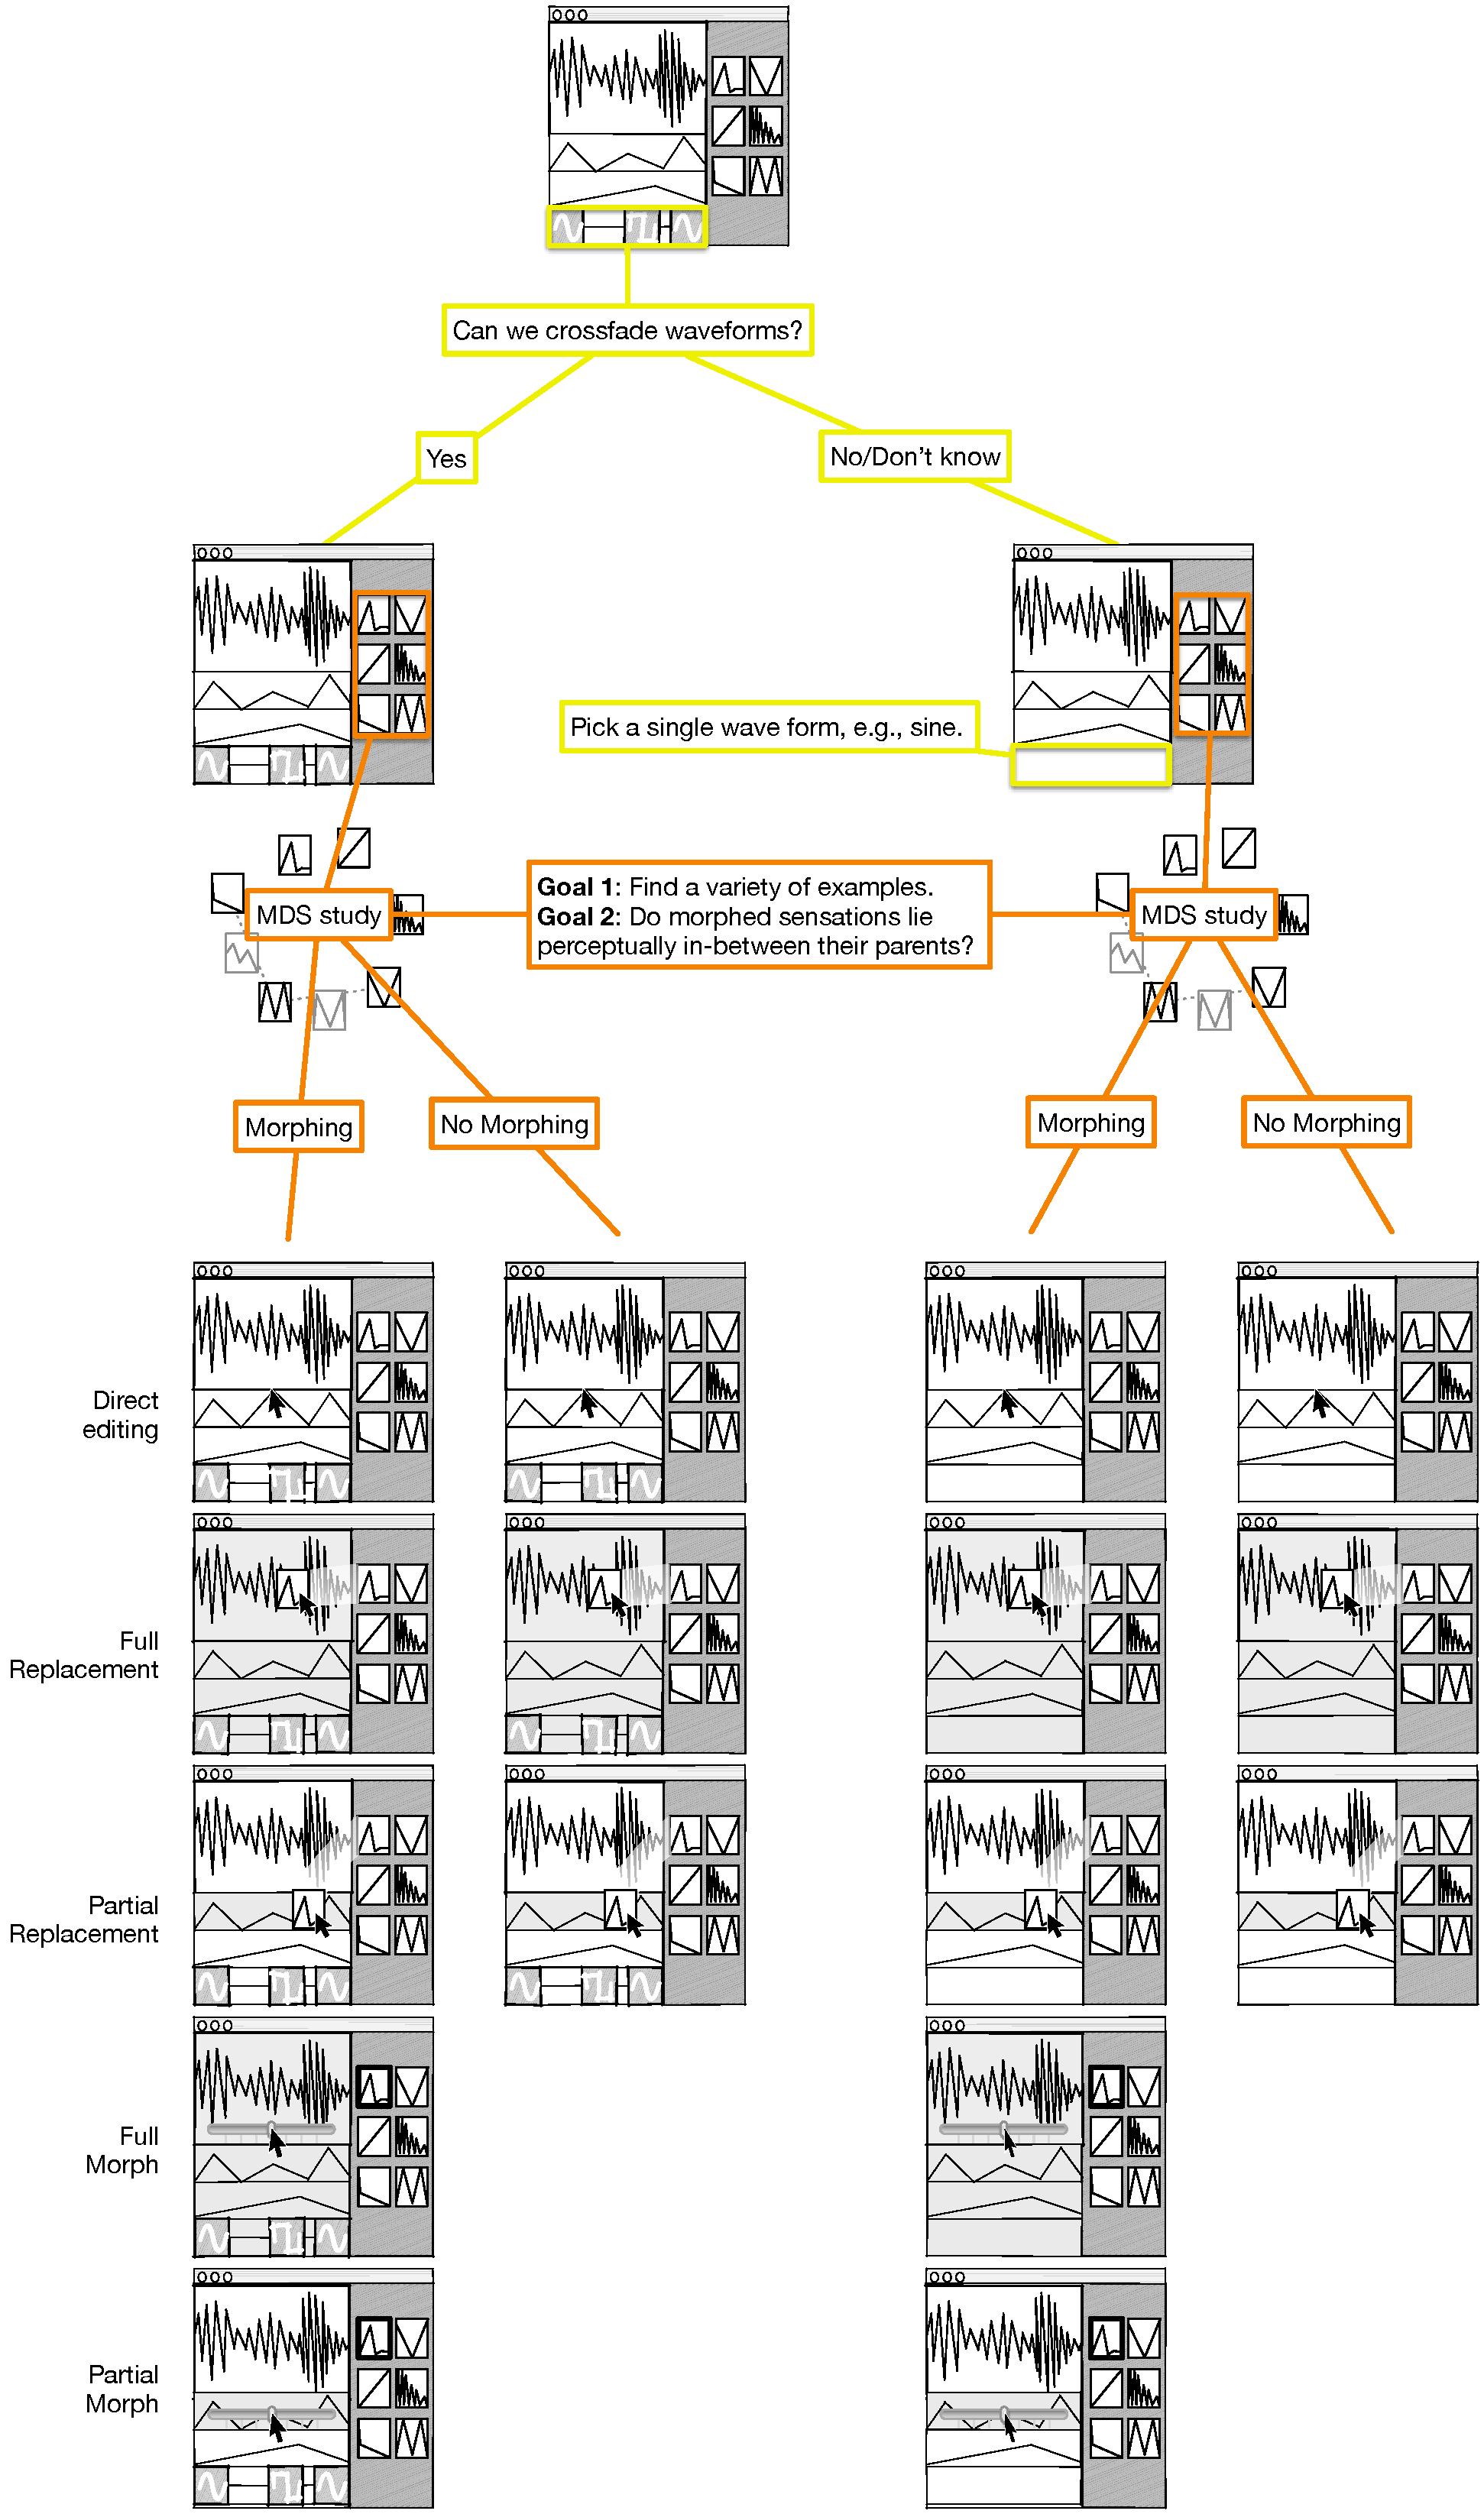
\includegraphics[width=0.7\textwidth, height=0.8\textheight]{HapticExamples-MorphingOrNot}

\caption{Phase I overview, with possible outcomes. We 1) pilot crossfading between waveforms, and 2) conduct an MDS study to find perceptually varied icons and evaluate morphing. The end result is a set of interaction techniques suitable for Phase II.}
\label{fig:macaron:phaseI:overview}
\end{center}
\end{figure}

\subsection{Morphing}
I propose to develop a \emph{morphing} algorithm for VT icons, based on dynamic time warping (DTW) of keyframes in each of the parameter tracks.
The goal is to have a linear, perceptually-smooth transition between VT icons that lets users mix examples, much like a painter might mix colours from a palette.
Similar to VT icon replacement, morphing could be between entire VT Icons (\emph{full morphing}), or between tracks (\emph{partial morphing}).

\subsection{Multidimensional Scaling Study}
To evaluate the morphing algorithm, and to develop a suitable set of VT icons for Phase II, I plan to conduct a multidimensional scaling (MDS) study.
MDS is a psychophysical technique that uses similarity scores between stimuli to build a visualization along underlying perceptual dimensions.
We can use this study to find two results:
\begin{enumerate}
\item From an initial set of 20-30 VT icons, we can identify clusters of similar icons, and select a diverse set of examples for Phase II.
\item By including a VT icons produced by the morphing algorithm, we can see whether they lie on a smooth perceptual path between their parent icons. If so, the morphing algorithm does indeed provide a perceptually smooth transition between parents. 
\end{enumerate}

The possible outcomes for Phase I are visualized in \autoref{fig:macaron:phaseI:overview}.



\section{Phase II -- Design Gallery Development and Evaluation}
In Phase II, I will develop a design tool that implements these algorithms, and use it to study how users involve examples in their designs.
An HTML/JavaScript prototype is under development (\autoref{fig:macaron:phaseII:prototype}), which generates sound that is streamed to the Haptuator through the audio jack.
Our questions and planned studies are visualized in \autoref{fig:macaron:phaseII:overview}.

\begin{figure}[h]
\centering
 \begin{subfigure}[t]{0.4\textwidth}
	\begin{center}
	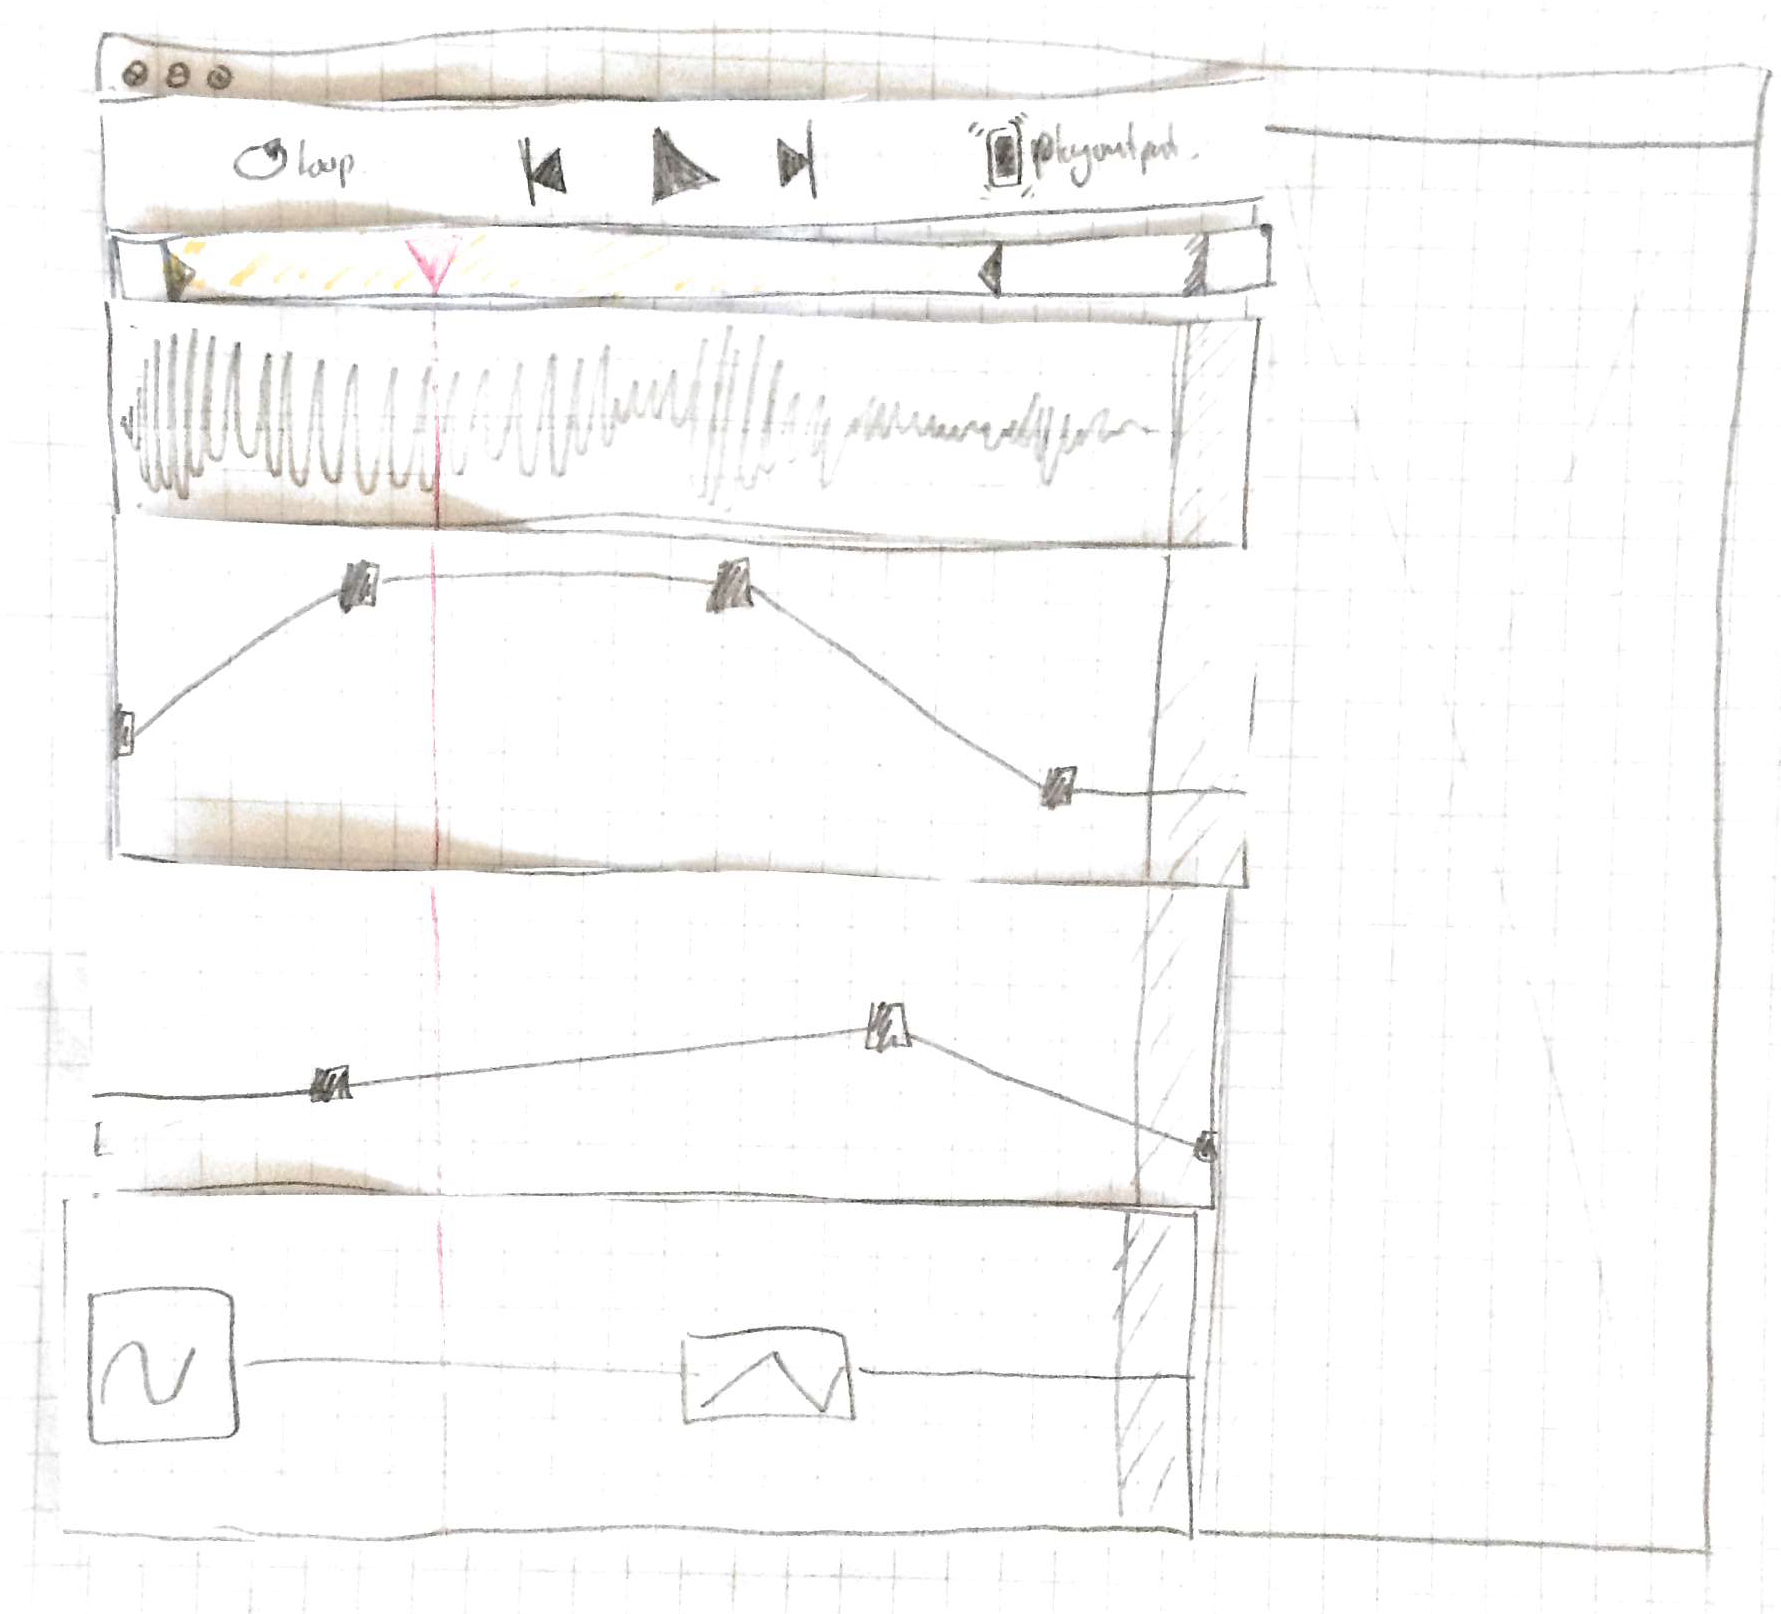
\includegraphics[width=\textwidth]{InitialMacaronEditorPaperPrototypeCropped}
	\caption{Paper prototype.}
	\label{fig:macaron:phaseII:prototype:paper}
	\end{center}
    \end{subfigure}
 ~
 \begin{subfigure}[t]{0.4\textwidth}
	\begin{center}
	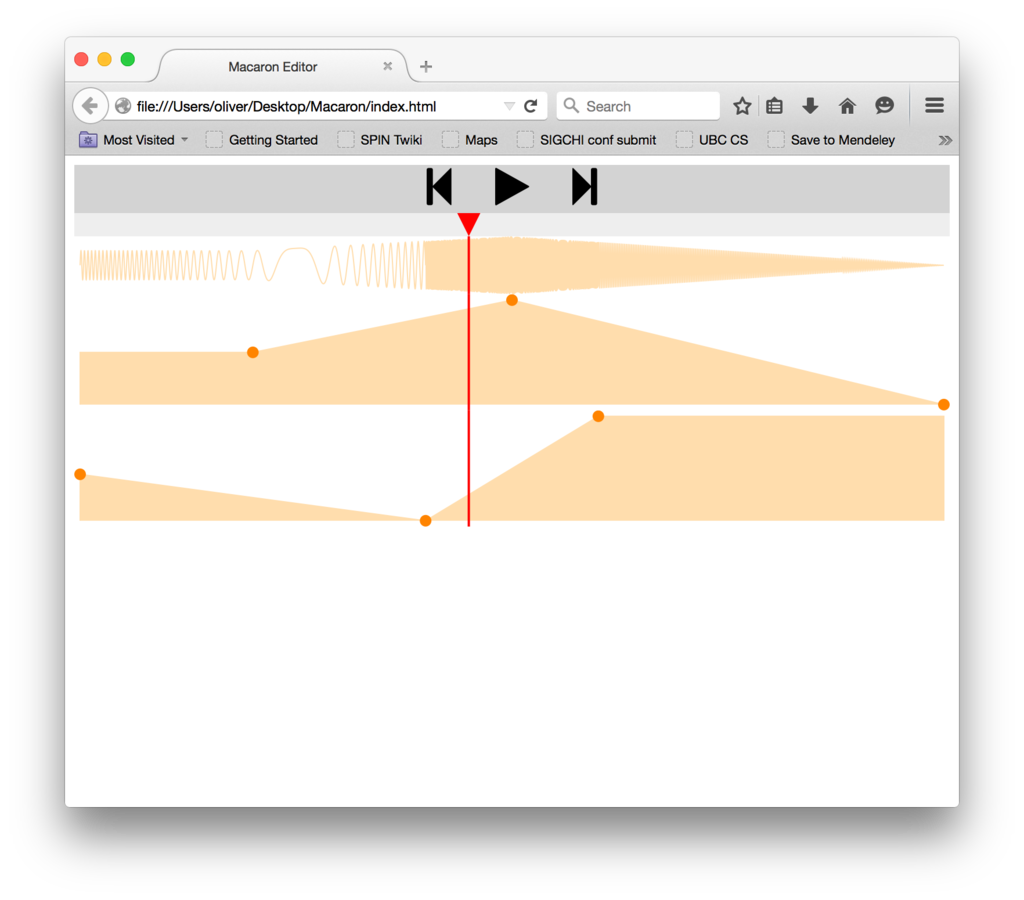
\includegraphics[width=\textwidth]{MacaronEditorScreenshot-2015-05-12}
	\caption{HTML/JavaScript prototype.}
	\label{fig:macaron:phaseII:prototype:html}
	\end{center}
    \end{subfigure}
	
	\caption{Initial prototypes for Macaron Editor.}
	\label{fig:macaron:phaseII:prototype}

\end{figure}




\section{Deliverables and Risk}

This project is intended to be completed in fall 2015, with a planned paper submission to CHI'16 or HAPTICS'16 (deadline in September), DIS'16 (deadline expected in December), or a similar venue.
I mitigate risk in following ways.
%However, given the number of side-projects scheduled in summer 2015, it's possible that this timeframe will be extended.
Phase I studies are designed to result in actionable results with or without waveform crossfading and morphing (\autoref{fig:macaron:phaseI:overview}).
If vibrotactile icons are not found to be diverse, I can select icons via piloting or from the HapTurk side project, which currently has a diverse set of icons selected.
Phase II studies are also designed to robustly provide results; we are primarily describing what users are doing.
If our system encounters technical problems, we can adjust the scope to mitigate risk, focusing more or less on Phase I or Phase II.
For example, if Phase II runs into unforeseen problems, we can submit a focused piece on Phase I (algorithms and interaction techniques) with more thorough investigation of morphing or waveform crossfading.
Alternatively, if Phase I encounters much difficulty, we can extend Phase II and look more at user interactions and less at algorithms.
Finally, if both Phases are compromised due to implementation problems, we can study these research questions by extending a previous tool: mHIVE, Mango, FeelCraft, and Feel Messenger could all be extended to investigate similar research questions.


\begin{figure}[htbp]
\begin{center}
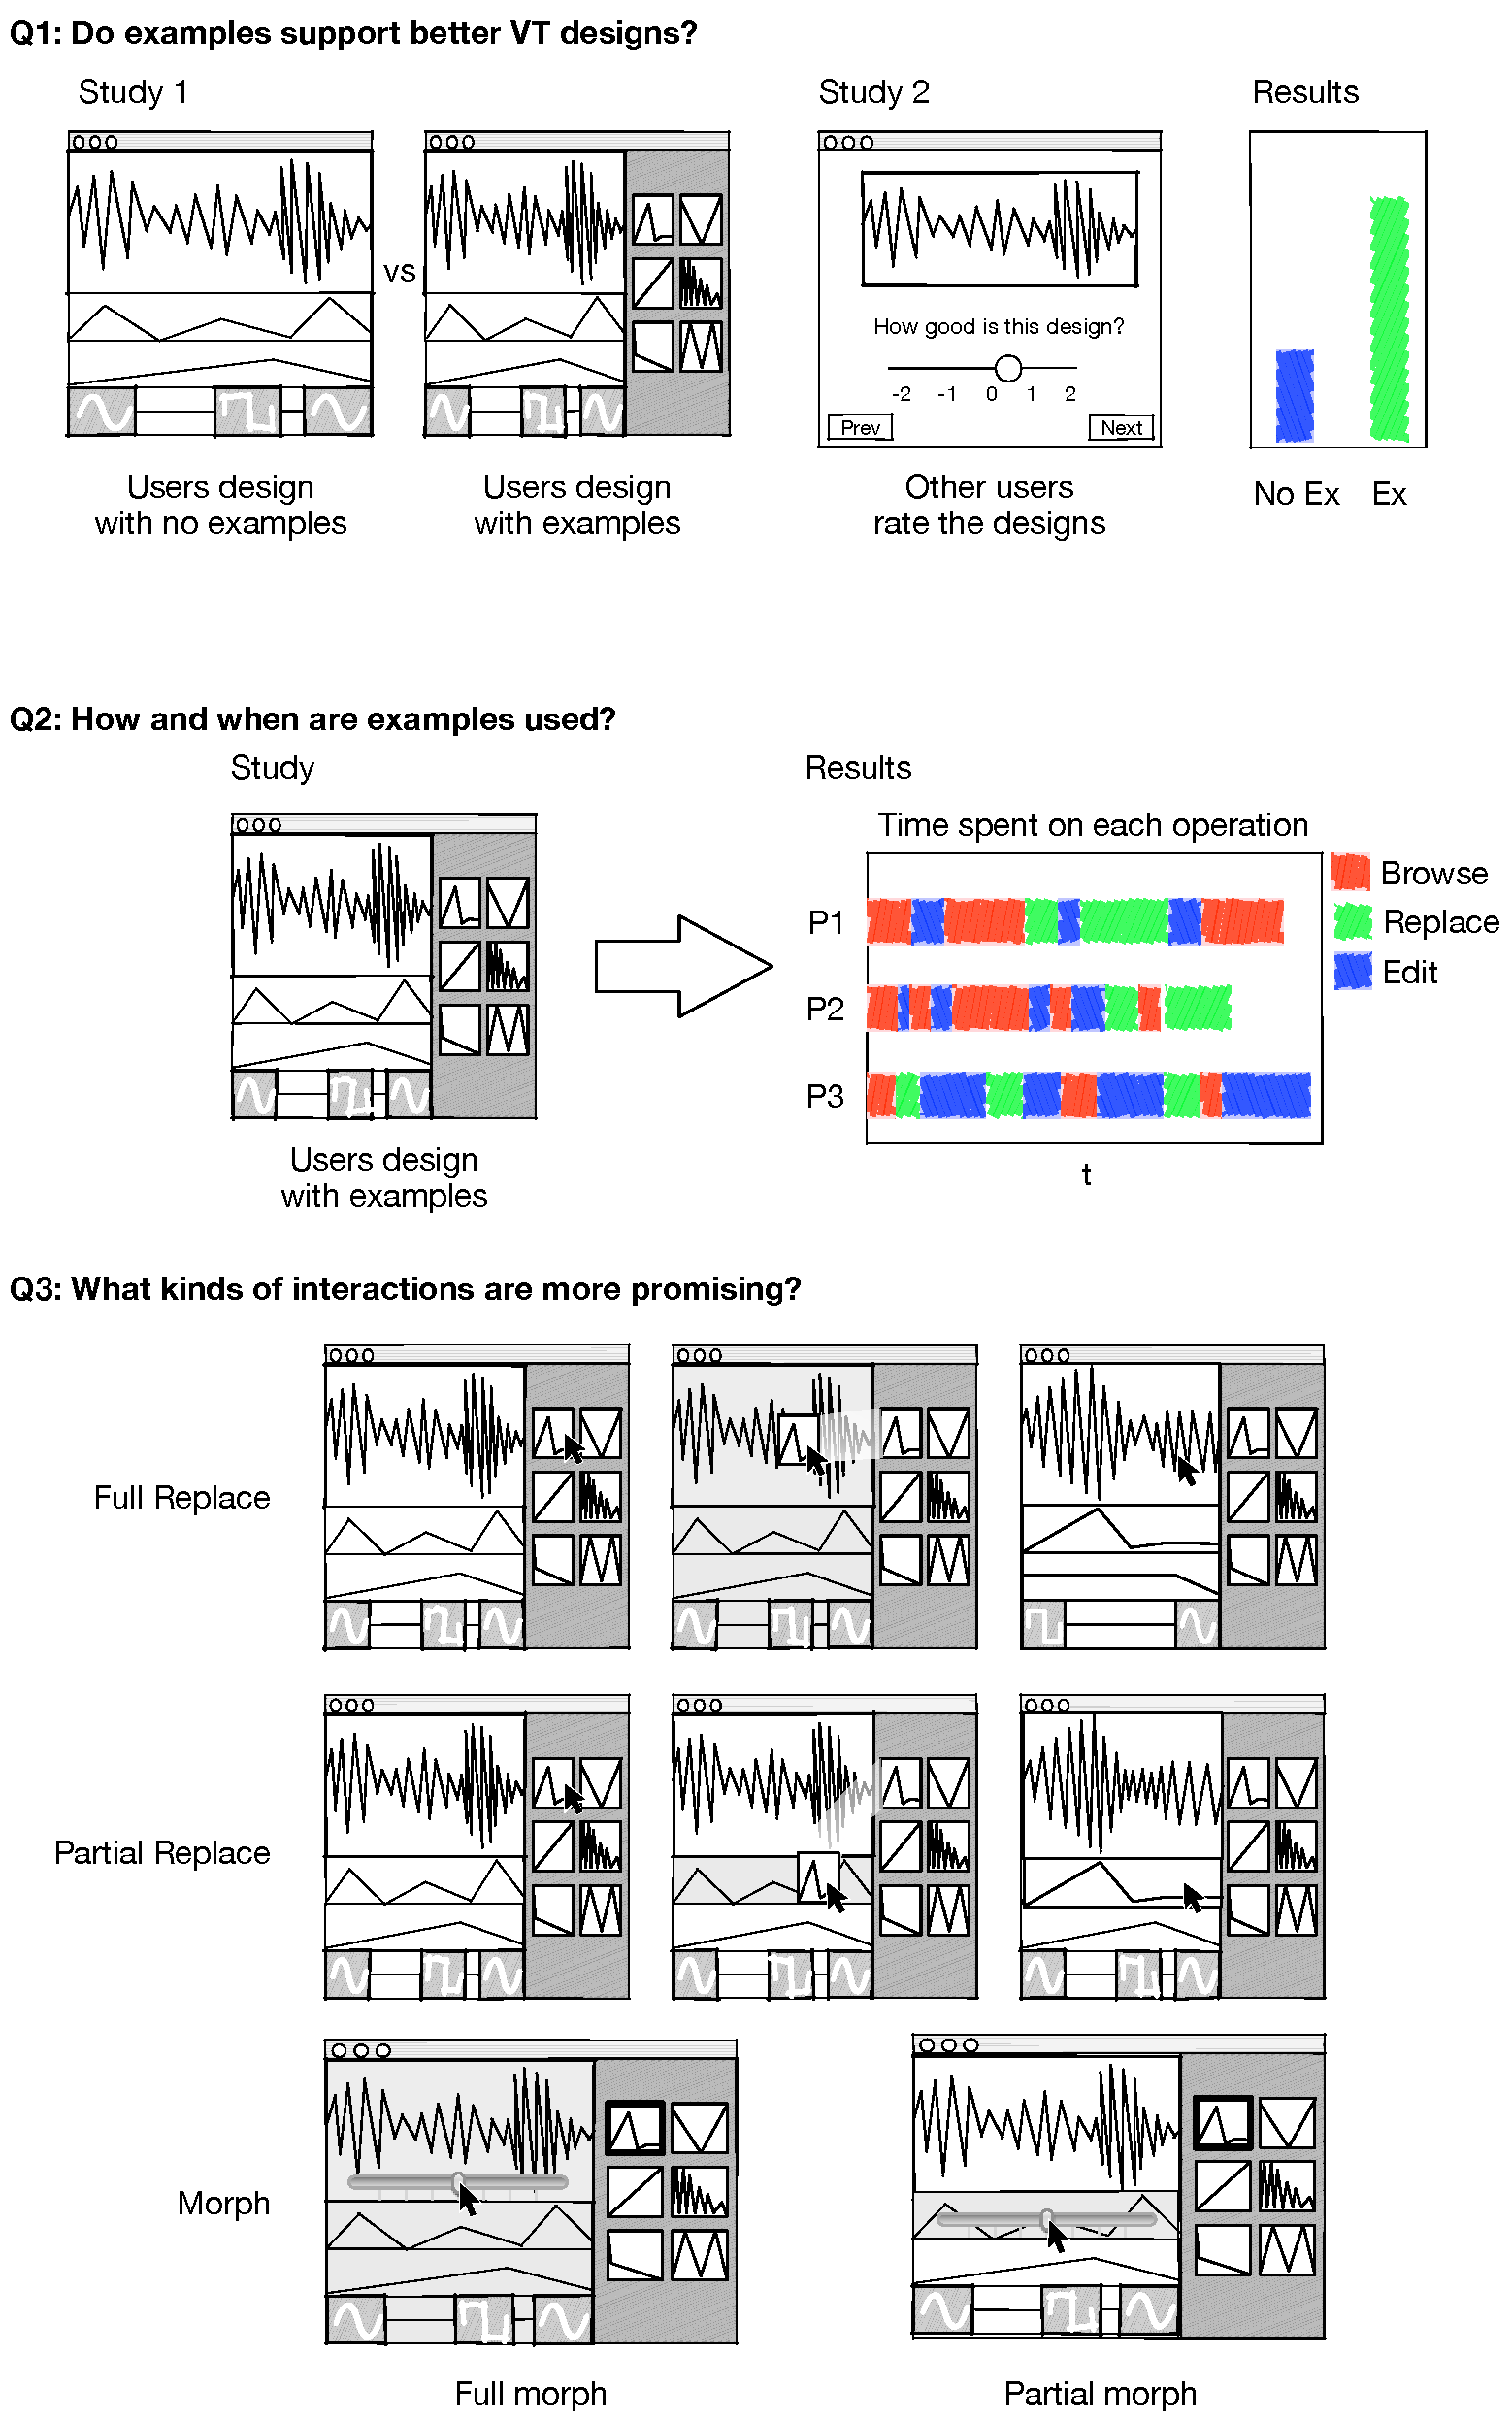
\includegraphics[width=0.7\textwidth, height=0.9\textheight]{DesignGalleryQuestions}

\caption{Phase II overview, split into research questions.}
\label{fig:macaron:phaseII:overview}
\end{center}
\end{figure}



%\begin{figure}[htbp]
%\begin{center}
%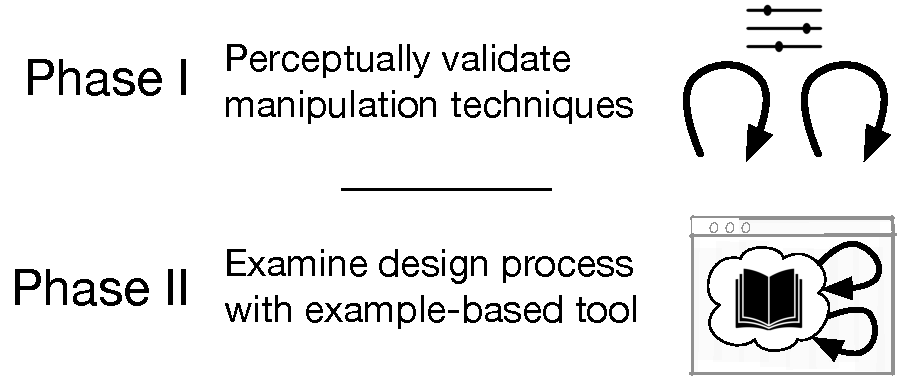
\includegraphics[width=0.8\textwidth]{ExamplesPhases}
%
%\caption{The two phases for the design gallery project.}
%\label{hapticexamples:phases}
%\end{center}
%\end{figure}



\endinput
